\setcounter{algorithm}{0}
\setcounter{figure}{0}
\setcounter{equation}{0}
\setcounter{theorem}{0}

\renewcommand{\thetheorem}{S\arabic{theorem}}
\renewcommand{\thelemma}{S\arabic{lemma}}
\renewcommand{\theequation}{S\arabic{equation}}
\renewcommand{\thefigure}{S\arabic{figure}}
\renewcommand{\thetable}{S\arabic{table}}
\renewcommand{\thealgorithm}{S\arabic{algorithm}}


\begin{center}
    \Large \textbf{Appendix: Algorithms, Proofs, and Numerical Results}
\end{center}

\section{Additional Algorithmic Details} \label{app:algorithms}

\subsection{Implementation of Alternative Methods}

\begin{algorithm}[!htb]
    \caption{Separate Prediction Intervals with Bonferroni Correction}
    \label{alg:bonferroni}
    \textbf{Input:} Calibration residuals $\{\mathbf{E}^i\}_{i=1}^{n}$; target miscoverage level $\alpha\in(0,1)$; test input $\mathbf{X}^{n+1}$.
    \begin{algorithmic}[1]
        \State Compute $\alpha^* \gets \alpha/d$.
        \For{$j=1$ to $d$}
        \State Compute $\hat{Q}_{1-\alpha^*,j} \gets \hat{Q}_{1-\alpha^*}(E^1_j,\ldots,E^n_j)$.
        \EndFor
        \State \Return $\hat{C}^{\mathrm{Bonf.}}(\mathbf{X}^{n+1}) \gets \left\{\mathbf y \in \R^d: 0 \leq E_j(\mathbf{X}^{n+1},y_j) \leq \hat{Q}_{1-\alpha^*,j}, \forall j \in [d]\right\}$.
    \end{algorithmic}
\end{algorithm}

\begin{algorithm}[!htb]
    \caption{Prediction Intervals via Dimension Reduction with $\ell_\infty$-Norm (Unscaled)}
    \label{alg:unscaled}
    \textbf{Input:} Calibration residuals $\{\mathbf{E}^i\}_{i=1}^{n}$; target miscoverage level $\alpha\in(0,1)$; test input $\mathbf{X}^{n+1}$.
    \begin{algorithmic}[1]
        \State Compute $S^i_{\mathrm{unscaled}} \gets \|\mathbf{E}^i\|_\infty$ for $i = 1,\ldots,n$.
        \State Compute $\hat{Q}^{\mathrm{unscaled}}_{1-\alpha} \gets \hat{Q}_{1-\alpha}(S^1_{\mathrm{unscaled}},\dots, S^n_{\mathrm{unscaled}})$
        \State \Return $\hat{C}^{\mathrm{unscaled}}(\mathbf{X}^{n+1}) \gets \left\{\mathbf y \in \R^d: 0 \leq E_j(\mathbf{X}^{n+1},y_j) \leq \hat{Q}^{\mathrm{unscaled}}_{1-\alpha}, \forall j \in [d]\right\}$.
    \end{algorithmic}
\end{algorithm}

\begin{algorithm}[!htb]
    \caption{Heuristic Plug-In Standardization}
    \label{alg:std-plug-in}
    \textbf{Input:} Calibration residuals $\{\mathbf{E}^i\}_{i=1}^{n}$; target miscoverage level $\alpha\in(0,1)$; test input $\mathbf{X}^{n+1}$.
    \begin{algorithmic}[1]
        \For{$j=1$ to $d$}
            \State Compute the location and scale parameters
            \begin{align*}
            & \hat{\mu}^{\mathrm{pi}}_j \gets \frac{1}{n}\sum_{i=1}^{n} E^i_j,
              & \hat{\sigma}^{\mathrm{pi}}_j \gets \sqrt{\frac{1}{n-1}\sum_{i=1}^{n}(E^i_j-\hat{\mu}^{\mathrm{pi}}_j)^2}.
            \end{align*}
            \EndFor
        \State Compute $S^i_{\mathrm{pi}} \gets \Phi(\mathbf{E}^i; \hat{\boldsymbol\mu}^{\mathrm{pi}},\hat{\boldsymbol\sigma}^{\mathrm{pi}})$ for $i \in [n]$, using $\Phi$ defined in~\eqref{eq:residual-transformation}.
        \State Compute $\hat{Q}^\mathrm{pi}_{1-\alpha}\gets \hat{Q}_{1-\alpha}(S^1_\mathrm{pi},\dots, S^n_\mathrm{pi}).$
        \State Compute 
            \begin{align*}
\hat{C}^{\mathrm{pi}}(\mathbf{X}^{n+1}) \gets \left\{\mathbf y \in \R^d: 0 \leq E_j(\mathbf{X}^{n+1}, y_j) \leq \hat{Q}^\mathrm{pi}_{1-\alpha}\cdot \hat{\sigma}^\mathrm{pi}_j + \hat{\mu}^\mathrm{pi}_j, \forall j \in [d]\right\},
            \end{align*}
            which is hyper-rectangular for the standard choices of $\mathbf E$ discussed in Section~\ref{sec:calibration}.
            \State \Return Prediction set $\hat{C}^{\mathrm{pi}}(\mathbf{X}^{n+1})$.
    \end{algorithmic}
\end{algorithm}

\begin{algorithm}[!htb]
    \caption{Standardization with Data Splitting}
    \label{alg:std-ds}
    \textbf{Input:} Calibration residuals $\{\mathbf{E}^i\}_{i=1}^{n}$; target miscoverage level $\alpha\in(0,1)$; test input $\mathbf{X}^{n+1}$.\\
    \textbf{Output:} $\hat{C}^{\mathrm{ds}}(\mathbf{X}^{n+1})$
    \begin{algorithmic}[1]
        \State Randomly split $\{1,\ldots,n\}$ into two disjoint subsets, $\mathcal{I}_1$ and $\mathcal{I}_2$.
        \For{$j=1$ to $d$}
            \State Compute the location and scale parameters
            \begin{align*}
            & \hat{\mu}^{\mathrm{ds}}_j \gets \frac{1}{|\mathcal{I}_1|}\sum_{i \in \mathcal I_1}E^i_j,
              & \hat{\sigma}^{\mathrm{ds}}_j \gets \sqrt{\frac{1}{|\mathcal I_1|-1}\sum_{i \in \mathcal I_1}(E^i_j-\hat{\mu}^{\mathrm{ds}}_j)^2}.
            \end{align*}
        \EndFor
        \State Compute $S^i_{\mathrm{ds}} \gets \Phi(\mathbf{E}^i; \hat{\boldsymbol\mu}^{\mathrm{ds}},\hat{\boldsymbol\sigma}^{\mathrm{ds}})$ for $i \in \mathcal I_2$, using $\Phi$ defined in~\eqref{eq:residual-transformation}.
        \State Compute $\hat{Q}^\mathrm{ds}_{1-\alpha}\gets \hat{Q}_{1-\alpha}(S^1_\mathrm{ds},\dots, S^n_\mathrm{ds}).$
        \State \Return $\hat{C}^{\mathrm{ds}}(\mathbf{X}^{n+1}) \gets \left\{\mathbf y \in \R^d: 0 \leq E_j(\mathbf{X}^{n+1}, y_j) \leq \hat{Q}^\mathrm{ds}_{1-\alpha}\cdot \hat{\sigma}^\mathrm{ds}_j + \hat{\mu}^\mathrm{ds}_j, \forall j \in [d]\right\}$.
    \end{algorithmic}
\end{algorithm}

\FloatBarrier

\subsection{Auxiliary Algorithms}

\begin{algorithm}[!htb]
\caption{Global-Worst-Case TSCP (TSCP-GWC)}
\label{alg:global}
\textbf{Input:} Calibration residuals $\{\mathbf{E}^i\}_{i=1}^{n}$; target miscoverage level $\alpha\in(0,1)$; test input $\mathbf{X}^{n+1}$.
\begin{algorithmic}[1]
\State Compute $\hat{\boldsymbol\mu}^{\mathrm{obs}}, \hat{\boldsymbol\sigma}^{\mathrm{obs}}$ using~\eqref{eq:plug-in-mean-std}.
\State Compute $S^i_{\mathrm{gwc}}\gets \hat{\Phi}^{\mathrm{gwc}}(\mathbf{E}^i)$ using $\hat{\Phi}^{\mathrm{gwc}}$ defined in Lemma~\ref{lem:gwc-rescaling}.
\State Compute $\hat{Q}^{\mathrm{gwc}}_{1-\alpha} \gets \hat{Q}_{1-\alpha}(S^1_{\mathrm{gwc}},\dots, S^n_{\mathrm{gwc}})$.
\State Compute $\omega_1(\hat{Q}^{\mathrm{gwc}}_{1-\alpha}),\ldots,\omega_d(\hat{Q}^{\mathrm{gwc}}_{1-\alpha})$ using $\omega$ defined in Lemma~\ref{lem:solution-key-ineq}.
\State \Return $\displaystyle \hat{C}^{\mathrm{gwc}}(\mathbf{X}^{n+1}) \gets \left\{\mathbf y\in \R^d: 0\leq E_j(\mathbf{X}^{n+1}, y_j) \leq  \omega_j(\hat{Q}^{\mathrm{gwc}}_{1-\alpha}), \forall j \in [d]\right\}$.
\end{algorithmic} 
\end{algorithm}

\begin{algorithm}[!htbp]
\caption{Backward Search in Algorithm~\ref{alg:shortcut}}
\label{alg:backward}
\textbf{Input:} Calibration residuals $\{\mathbf{E}^i\}_{i=1}^{n}$; global bounds $\omega_1(\hat{Q}^{\mathrm{gwc}}_{1-\alpha}),\ldots,\omega_d(\hat{Q}^{\mathrm{gwc}}_{1-\alpha})$; target miscoverage level $\alpha\in(0,1)$; calibration mean $\hat{\boldsymbol\mu}^{\mathrm{obs}}$ and standard deviation $\hat{\boldsymbol\sigma}^{\mathrm{obs}}$; mean index $h^*$; current coordinate $j$.
\begin{algorithmic}[1]
    \For{$h\in \mathrm{Row}_j(h^*)$ with $h_j=h^*_j-1$ to $1$}
        \State Compute $\omega_j(\hat{Q}^{\mathrm{lwc}}_{1-\alpha}(\mathcal{Y}^h))$ using Algorithm~\ref{alg:local-bound} and $B^{h}_j$ using~\eqref{eq:rect-wise-bounds}.
        \If{$B^{h}_j > 0$}
            \State \Return $h^{[j]} = h$.
        \EndIf
    \EndFor
\end{algorithmic}
\end{algorithm}

\begin{algorithm}[!htb]
\caption{Binary Search in Algorithm~\ref{alg:shortcut}}
\label{alg:binary}
\textbf{Input:} Calibration residuals $\{\mathbf{E}^i\}_{i=1}^{n}$; global bounds $\omega_1(\hat{Q}^{\mathrm{gwc}}_{1-\alpha}),\ldots,\omega_d(\hat{Q}^{\mathrm{gwc}}_{1-\alpha})$; target miscoverage level $\alpha\in(0,1)$; calibration mean $\hat{\boldsymbol\mu}^{\mathrm{obs}}$ and standard deviation $\hat{\boldsymbol\sigma}^{\mathrm{obs}}$; mean index $h^*$; current coordinate $j$.
\begin{algorithmic}[1]
    \State Let $I_{\min} \gets h^*_j$ and $I_{\max} \gets n+1$.
    \While{$I_{\min} < I_{\max}$}
        \State Compute $m_j\gets \lceil (I_{\mathrm{min}}+I_\mathrm{max})/2\rceil$ and $m_k = h^*_k$ for all $k\neq j$.
        \State Compute $\omega_j(\hat{Q}^{\mathrm{lwc}}_{1-\alpha}(\mathcal{Y}^m))$ and $B^{m}_j$ using~\eqref{eq:rect-wise-bounds}.\hfill
        \Comment{Algorithm~\ref{alg:local-bound}}
        \If{$B^{m}_j > 0$}
            \State $I_{\mathrm{min}} \gets m_j$.
        \Else 
            \State $I_{\mathrm{max}} \gets m_j-1$.
        \EndIf
        \If{$I_{\max} = I_{\min}$}
            \State \Return $h^{[j]}_j = I_{\min}$ and $h^{[j]}_k = h^*_k$ for all $k\neq j$.
        \EndIf
    \EndWhile
\end{algorithmic}
\end{algorithm}


\FloatBarrier

\subsection{Computational Cost Analysis}\label{app:alg-and-cost}

\subsubsection{Algorithm~\ref{alg:global}}
\label{app:gwc-cost}
Since the calibration residuals $\{\mathbf{E}^i\}_{i=1}^{n}$ are stored as an $(n,d)$-array, we know
\begin{enumerate}
    \item Computing $(\hat\mu^{\mathrm{obs}}_j,\hat\sigma^{\mathrm{obs}}_j)_{j=1}^d$ using~\eqref{eq:plug-in-mean-std} requires $\mathcal O(nd)$.
    \item Evaluating $S^i_{\mathrm{gwc}}\gets \hat{\Phi}^{\mathrm{gwc}}(\mathbf{E}^i)$ for all $i\in[n]$ is also $\mathcal O(nd)$.
    \item Computing the quantile $\hat{Q}^{\mathrm{gwc}}_{1-\alpha}$ costs $\mathcal O(n)$ using a selection algorithm such as quickselect. 
    \item Computing $\omega_1(\hat{Q}^{\mathrm{gwc}}_{1-\alpha}),\ldots,\omega_d(\hat{Q}^{\mathrm{gwc}}_{1-\alpha})$ costs $\mathcal{O}(d)$ once $\hat{Q}^{\mathrm{gwc}}_{1-\alpha}$ and $(\hat\mu^{\mathrm{obs}}_j,\hat\sigma^{\mathrm{obs}}_j)_{j=1}^d$ are known.
\end{enumerate}
Hence, the overall computational complexity of Algorithm~\ref{alg:global} is $\mathcal O(nd)$.

\subsubsection{Algorithm~\ref{alg:local-bound}}
\label{app:lwc-local-bound}

Algorithm~\ref{alg:local-bound} shares the same structure and computational cost as Algorithm~\ref{alg:global}: $\mathcal O(nd)$.

\subsubsection{Algorithm~\ref{alg:shortcut}}
\label{app:lwc-sc-cost}
Since the calibration residuals $\{\mathbf{E}^i\}_{i=1}^{n}$ are stored as an $(n,d)$-array, we know
\begin{enumerate}
    \item Computing $(\hat\mu^{\mathrm{obs}}_j,\hat\sigma^{\mathrm{obs}}_j)_{j=1}^d$ using~\eqref{eq:plug-in-mean-std} and $\omega_1(\hat{Q}^{\mathrm{gwc}}_{1-\alpha}),\ldots,\omega_d(\hat{Q}^{\mathrm{gwc}}_{1-\alpha})$ using Algorithm~\ref{alg:global} requires $\mathcal O(nd)$.
    \item Sorting $\{E^i_j\}^n_{i=1}$ for all $j\in [d]$ costs $\mathcal{O}(dn\log{n})$;
    \item Computing $\mathcal{Y}^{h^*}$ relies on computing $h^*$, which requires masking all values below $\hat{\boldsymbol\mu}^{\mathrm{obs}}$ and reporting the index of the lowest value from the sorted residuals list $\{E^i_j\}^n_{i=1}$, each of which costs $\mathcal{O}(n)$, so together this operation contributes $\mathcal{O}(dn)$.
    \item If $\mathcal{Y}^{h^*} = \emptyset$, then the cost is only $\mathcal{O}(d)$ since all global bounds have been computed.
    \item If $\mathcal{Y}^{h^*} \neq \emptyset$, then for each coordinate, we compute the local bounds using Algorithm~\ref{alg:local-bound} and $B^{h^*}_j$ using~\eqref{eq:rect-wise-bounds}, which costs $\mathcal{O}(dn)$.
    If $B^{h^*}_j = 0$, then we use the backward search detailed in Algorithm~\ref{alg:backward}, which costs $\mathcal{O}(dn^2)$; see Appendix~\ref{app:backward-backward}.
    If $B^{h^*}_j > 0$, then we use the binary search detailed in Algorithm~\ref{alg:binary}, which costs $\mathcal{O}(dn\log{n})$; see Appendix~\ref{app:backward-binary}.
\end{enumerate}  
Let $T \leq d$ be the number of coordinates where binary searches are enabled, then the total cost of Algorithm~\ref{alg:shortcut} is $\mathcal{O}(Tdn\log{n} + (d-T)dn^2)$.

\subsubsection{Algorithm~\ref{alg:backward}} \label{app:backward-backward}
Running Algorithm~\ref{alg:local-bound} and forming $B^h_j$ costs $\mathcal{O}(dn)$ for each $h$; there are $n+1$ indices in
$\mathrm{Row}_j(h^*)$, so the computational complexity of Algorithm~\ref{alg:backward} never exceeds $\mathcal{O}(dn^2)$.

\subsubsection{Algorithm~\ref{alg:binary}} \label{app:backward-binary}
Running Algorithm~\ref{alg:local-bound} and forming $B^h_j$ costs $\mathcal{O}(dn)$ for each $h$. The number of indices $h$ encountered in this algorithm is $\mathcal{O}(\log_2{n})$ because we split and continue in only half of the current indices sequence at each step. This is a standard binary search. Therefore, the total computational complexity of Algorithm~\ref{alg:binary} never exceeds $\mathcal{O}(dn\log{n})$.

\clearpage

\section{Mathematical Proofs} 
\label{app:proofs}

\subsection{Auxiliary Lemmas}\label{app:proofs-lemmas}

\begin{lemma}\label{lem:1}
    Let $x^1,\ldots,x^n \in \R$ and $\bar{x}^n = \frac{1}{n}\sum^n_{i=1}x^i$. For any $x^{n+1}\in \R$, let $\hat\sigma(x^{n+1})$ be the sample standard deviation of $\{x^1,\ldots,x^n, x^{n+1}\}$, then
    \[
    \hat\sigma^2(x^{n+1}) = \frac{(x^{n+1}-\bar{x}^{n})^2}{n+1}+\frac{1}{n}\sum^n_{i=1}(x^i-\bar{x}^{n})^2.
    \]
\end{lemma}
\begin{proof}
    Denote $\bar{x}^{n+1} = \frac{1}{n+1}\sum^{n+1}_{i=1}x^i$. We notice that
\begin{align*}
    \hat\sigma^2(x^{n+1}) = &\frac{1}{n}\sum^{n+1}_{i=1}(x^i-\bar{x}^{n+1})^2\\
    = &\frac{1}{n} \left[ (x^{n+1}-\bar{x}^{n+1})^2+\sum^n_{i=1}(x^i-\bar{x}^{n}+\bar{x}^{n}-\bar{x}^{n+1})^2 \right]\\
    = &\frac{(x^{n+1}-\bar{x}^{n+1})^2}{n}+\frac{1}{n}\sum^n_{i=1}\left[(x^i-\bar{x}^{n})^2+2(x^i-\bar{x}^n)(\bar{x}^n-\bar{x}^{n+1})+(\bar{x}^{n}-\bar{x}^{n+1})^2\right]\\
    = &\frac{(x^{n+1}-\bar{x}^{n+1})^2}{n}+(\bar{x}^{n}-\bar{x}^{n+1})^2+\frac{1}{n}\sum^n_{i=1}(x^i-\bar{x}^{n})^2.
\end{align*}
Substituting $\bar{x}^{n+1} = \frac{x^{n+1}+n\bar{x}^n}{n+1}$, we get
\begin{align*}    
    \hat\sigma^2(x^{n+1}) = &\frac{1}{n}\left(x^{n+1}-\frac{x^{n+1}+n\bar{x}^n}{n+1}\right)^2+\left(\bar{x}^n-\frac{n\bar{x}^n+x^{n+1}}{n+1}\right)^2+\frac{1}{n}\sum^n_{i=1}(x^i-\bar{x}^{n})^2\\
    = &\frac{n}{(n+1)^2}(x^{n+1}-\bar{x}^n)^2+\frac{1}{(n+1)^2}(\bar{x}^n-x^{n+1})^2+\frac{1}{n}\sum^n_{i=1}(x^i-\bar{x}^{n})^2\\
    = &\frac{(x^{n+1}-\bar{x}^{n})^2}{n+1}+\frac{1}{n}\sum^n_{i=1}(x^i-\bar{x}^{n})^2.
\end{align*}
\end{proof}

\begin{lemma}\label{lem:2}
    Let $X^1,\ldots, X^n \in \R$ be real-valued random variables with sample mean $\bar{X}^n$. Let $X^{n+1}$ and $\tilde{X}^{n+1}$ be another two random variables such that
    \[
    |X^{n+1} - \bar{X}^n| \leq |\tilde{X}^{n+1}-\bar{X}^n| \quad \text{a.s.}
    \]
    Then,
    \[
    \hat{\sigma}(X^{n+1}) \leq \hat{\sigma}(\tilde{X}^{n+1}) \quad \text{a.s.},
    \]
    where $\hat{\sigma}(X^{n+1})$ is the sample standard deviation of $\{X^1,\ldots,X^n, X^{n+1}\}$, as in Lemma~\ref{lem:1}.
\end{lemma}
\begin{proof}
    This is a direct application of Lemma~\ref{lem:1}:
\begin{align*}
    \hat{\sigma}^2(X^{n+1}) 
    &= \frac{(X^{n+1}-\bar{X}^{n})^2}{n+1}+\frac{1}{n}\sum^n_{i=1}(X^i-\bar{X}^{n})^2\\
    &\leq \frac{(\tilde{X}^{n+1}-\bar{X}^{n})^2}{n+1}+\frac{1}{n}\sum^n_{i=1}(X^i-\bar{X}^{n})^2 \quad \text{[Assumption]}\\
    &=\hat{\sigma}^2(\tilde{X}^{n+1}),
\end{align*}
and the claim follows by taking square roots.
\end{proof}


\begin{lemma}\label{lem:3}
    Let $X^1,\ldots, X^{n+1} \in \R$ be real-valued random variables with sample mean $\bar{X}^{n+1}$ and sample standard deviation $\bar{S}^{n+1} > 0$. Define $Z^i = (X^i-\bar{X}^{n+1}) / \bar{S}^{n+1}$ for $i \in [n+1]$. Then,
    \[
    |Z^i| \leq \frac{n}{\sqrt{n+1}} \quad\text{almost surely}, \quad \forall i \in [n+1].
    \]
    This inequality is strict if $X^1,\ldots,X^{n+1}$ are almost-surely distinct.
\end{lemma}
\begin{proof}
Fix any $i\in [n+1]$.
Let $\bar{X}^{-i} = \frac{1}{n}\sum_{k\neq i}X^k$ be the sample mean of the random variables excluding the $i$-th one, and
\[
\bar{S}^{-i} = \sqrt{\frac{1}{n}\sum_{k\neq i}(X^k - \bar{X}^{-i})^2}.
\]
Then, it follows from Lemma~\ref{lem:1} that
\[
|Z^i| = \frac{|X^i-\bar{X}^{n+1}|}{\bar{S}^{n+1}}
    = \frac{\left|X^i - \frac{1}{n+1}\sum^{n+1}_{k=1}X^k\right|}{\sqrt{\frac{1}{n}\sum^{n+1}_{k=1}(X^k - \bar{X}^{n+1})^2}}=\frac{\frac{n}{n+1}|X^i - \bar{X}^{-i}|}{\sqrt{\frac{1}{n+1}(X^i-\bar{X}^{-i})^2+(\bar{S}^{-i})^2}}.
\]
But $\bar{S}^{-i} \geq 0$, so we must have
\begin{align*}
    |Z^i|\leq \frac{\frac{n}{n+1}|X^i - \bar{X}^{-i}|}{\sqrt{\frac{1}{n+1}(X^i-\bar{X}^{-i})^2}}= \frac{n}{\sqrt{n+1}}.
\end{align*}
If $X^1,\ldots,X^{n+1}$ are almost-surely distinct, we know $\bar{S}^{-i} >0$ almost-surely for any $i \in [n+1]$ thus this inequality becomes strict.
\end{proof}


\subsection{Proofs of Main Results}
\label{app:proofs-thms}

\begin{proof}[of Theorem~\ref{thm:fixed-transformation-coverage}]
This is a well-known result, whose proof is included for completeness. 
By definition of $\hat{C}(\mathbf{X}^{n+1})$ in~\eqref{eq:joint-prediction-scalar},
\[
 \mathbf{Y}^{n+1} \notin \hat{C}(\mathbf{X}^{n+1}) \Longleftrightarrow S^{n+1} > \hat{Q}_{1-\alpha}(S^1,\ldots,S^n).
\]
Moreover, $S^1,\ldots,S^{n+1}$ are exchangeable because $\mathbf{E}^1,\ldots,\mathbf{E}^{n+1}$ are exchangeable and $\Phi$ is fixed.
Therefore, the proof is complete by applying the fundamental ``quantile inflation lemma'' of conformal prediction (e.g., see \citet{angelopoulos2025theoreticalfoundationsconformalprediction}), which states 
\begin{align*}
  \mathbb{P}\left[ S^{n+1} > \hat{Q}_{1-\alpha}(S^1,\ldots,S^n) \right] \leq \alpha.
\end{align*}
Moreover, it is also a standard result that, if $S^1,\ldots,S^{n+1}$ are almost-surely distinct,
\begin{align*}
  \mathbb{P}\left[ S^{n+1} > \hat{Q}_{1-\alpha}(S^1,\ldots,S^n) \right] \geq \alpha - \frac{1}{n+1}.
\end{align*}
\end{proof}

\begin{proof}[of Lemma~\ref{lem:solution-key-ineq}]
From Assumption~\ref{eq:assumption-scores}, we know that $E^1_j,\dots, E^{n+1}_j$ are almost-surely distinct for every $j \in [d]$ and $0<\hat{\sigma}^{\mathrm{oracle}}_j < \infty$ almost-surely for all $j \in [d]$, which also ensures $S_{\mathrm{oracle}}^{n+1}$ is well-defined. 
To prove this lemma, fix any $c \in \R$ and note that
\begin{align*}
    &S_{\mathrm{oracle}}^{n+1} \leq c \\
    &\iff E^{n+1}_j \leq c\,\hat{\sigma}^{\mathrm{oracle}}_j + \hat{\mu}^{\mathrm{oracle}}_j, \quad \forall j \in [d]\\
    &\iff {E^{n+1}_j - c\sqrt{\frac{1}{n}\sum^{n+1}_{i=1}\left(E^i_j -\frac{1}{n+1}\sum^{n+1}_{i=1}E^i_j, \right)^2} - \frac{1}{n+1}\sum^{n+1}_{i=1}E^i_j} \leq 0, \quad \forall j \in [d]\\
    &\iff {\frac{n}{n+1}\left(E^{n+1}_j-\hat{\mu}^\mathrm{obs}_j\right) - c\sqrt{\frac{1}{n}\sum^{n+1}_{i=1}\left(E^i_j -\frac{1}{n+1}\sum^{n+1}_{i=1}E^i_j, \right)^2}} \leq 0, \quad \forall j \in [d]\\
    &\iff \underbrace{\frac{n}{n+1}\left(E^{n+1}_j-\hat{\mu}^\mathrm{obs}_j\right) - c\sqrt{\frac{1}{n+1}\left(E^{n+1}_j-\hat{\mu}^\mathrm{obs}_j\right)^2+(\hat{\sigma}^\mathrm{obs}_j)^2}}_{=: g_j(\mathbf{E}^{n+1})} \leq 0, \quad \forall j \in [d]
\end{align*}
where the last implication follows from Lemma~\ref{lem:1}.
Everything except $\mathbf{E}^{n+1}$ here is observed, so we can solve this inequality for $\mathbf{E}^{n+1}$ coordinate-wise.

Fix any $j\in [d]$. It follows from the above that
\begin{align}
    g_j(\mathbf{E}^{n+1}) \leq 0 \iff \frac{n}{n+1}\left(E^{n+1}_j-\hat{\mu}^\mathrm{obs}_j\right) \leq c\sqrt{\frac{1}{n+1}\left(E^{n+1}_j-\hat{\mu}^\mathrm{obs}_j\right)^2+(\hat{\sigma}^\mathrm{obs}_j)^2}.
    \label{eq:coordinte-wise-key-ineq}
\end{align}
The solution of this inequality in $E^{n+1}_j$ depends on the range of $c$. There are two cases:
\begin{enumerate}
\item if $c \geq 0$, then~\eqref{eq:coordinte-wise-key-ineq} holds if and only if \emph{either} $0\leq E^{n+1}_j < \hat{\mu}^\mathrm{obs}_j$ \emph{or} $E^{n+1}_j \geq \hat{\mu}^\mathrm{obs}_j$ and
    \[
    \left(\frac{n}{n+1}\right)^2\left(E^{n+1}_j-\hat{\mu}^\mathrm{obs}_j\right)^2 \leq c^2\left(\frac{1}{n+1}(E^{n+1}_j-\hat{\mu}^\mathrm{obs}_j)^2 + (\hat{\sigma}^\mathrm{obs}_j)^2\right).
    \]
\item if $c < 0$, then~\eqref{eq:coordinte-wise-key-ineq} holds if and only if $E^{n+1}_j <  \hat{\mu}^\mathrm{obs}_j$ \emph{and}
    \begin{align*}
        \left(\frac{n}{n+1}\right)^2\left(E^{n+1}_j-\hat{\mu}^\mathrm{obs}_j\right)^2 \geq c^2\left(\tfrac{1}{n+1}\left(E^{n+1}_j-\hat{\mu}^\mathrm{obs}_j\right)^2 + (\hat{\sigma}^\mathrm{obs}_j)^2\right).
    \end{align*}
  \end{enumerate}
  The solution in both cases relies on solving a quadratic equality in the form $h(x) = 0$, where:
\[
h(x):=\left(\frac{n}{n+1}\right)^2\left(x-\hat{\mu}^\mathrm{obs}_j\right)^2 - c^2\tfrac{1}{n+1}\left(x-\hat{\mu}^\mathrm{obs}_j\right)^2 - c^2(\hat{\sigma}^\mathrm{obs}_j)^2 = 0.
\]
This equality can be reorganized into a more recognized quadratic form 
\[
h(x)= Ax^2+Bx +K = 0,
\]
where
\begin{align*}
 A & = \left(\frac{n}{n+1}\right)^2 - \frac{c^2}{n+1}, \\
 B & = 2\hat{\mu}^\mathrm{obs}_j\left(\frac{n}{n+1}\right)^2-2\hat{\mu}^\mathrm{obs}_j \frac{c^2}{n+1}, \\
 K & = \left(\frac{n}{n+1}\right)^2(\hat{\mu}^\mathrm{obs}_j)^2-\frac{c^2}{n+1}(\hat{\mu}^\mathrm{obs}_j)^2-c^2(\hat{\sigma}^\mathrm{obs}_j)^2.
\end{align*}
The solution set is:
\[h(x) = 0 \iff x=
\begin{cases}
    \hat{\mu}^\mathrm{obs}_j \pm \hat{\sigma}^\mathrm{obs}_j|c|\sqrt{\tfrac{(n+1)^2}{n^2-(n+1)c^2}}, & c^2 < \tfrac{n^2}{n+1},\\
    \hat{\mu}^\mathrm{obs}_j, & c^2 = \tfrac{n^2}{n+1} \text{ and } \hat{\sigma}^\mathrm{obs}_j = 0,\\
    \text{no real solution}, &\text{otherwise}.
\end{cases}
\]
We first note the event $\hat{\sigma}^\mathrm{obs}_j = 0$ occurs if and only if $E^1_j=\ldots=E^n_j$, which has probability zero by Assumption~\ref{eq:assumption-scores}. For the rest, we note that $c^2 < \tfrac{n^2}{n+1}$ implies $A>0$ thus $h(x) = Ax^2+Bx +K$ concave up for all $x \geq 0$. 
Therefore by analyzing the positiveness and negativeness of $h(x)$ relative to the solution set in our two cases, we know~\eqref{eq:coordinte-wise-key-ineq} holds almost-surely if and only if
\begin{align*}
    &\begin{cases}
    \hat{\mu}^\mathrm{obs}_j \leq E^{n+1}_j \leq \hat{\mu}^\mathrm{obs}_j+\hat{\sigma}^\mathrm{obs}_j|c|\sqrt{\tfrac{(n+1)^2}{n^2-(n+1)c^2}}, & c \geq 0,\, c^2 < \tfrac{n^2}{n+1}, \\[0.5em]
    E^{n+1}_j < \infty , & c \geq 0,\, c^2 \geq \tfrac{n^2}{n+1}, \\[0.5em]
    0 \leq E^{n+1}_j < \hat{\mu}^\mathrm{obs}_j, & c \geq 0, \\[0.5em]
    0\leq E^{n+1}_j \leq \hat{\mu}^\mathrm{obs}_j-\hat{\sigma}^\mathrm{obs}_j|c|\sqrt{\tfrac{(n+1)^2}{n^2-(n+1)c^2}}, & c < 0,\, c^2 < \tfrac{n^2}{n+1}, \\[0.5em]
    \text{no solution}, & c < 0,\, c^2 \geq \tfrac{n^2}{n+1}.
    \end{cases} \quad \text{almost-surely}\\
    &\iff \begin{cases}
    0 \leq E^{n+1}_j \leq \hat{\mu}^\mathrm{obs}_j+\hat{\sigma}^\mathrm{obs}_j|c|\sqrt{\tfrac{(n+1)^2}{n^2-(n+1)c^2}}, & 0\leq c < \tfrac{n}{\sqrt{n+1}}, \\[0.5em]
    0\leq E^{n+1}_j < \infty , & c\geq\tfrac{n}{\sqrt{n+1}}, \\[0.5em]
    0\leq E^{n+1}_j \leq \max\left\{0, \hat{\mu}^\mathrm{obs}_j-\hat{\sigma}^\mathrm{obs}_j|c|\sqrt{\tfrac{(n+1)^2}{n^2-(n+1)c^2}}\right\}, & -\tfrac{n}{\sqrt{n+1}} < c<0, \\[0.5em]
    \text{no solution}, & c \leq - \tfrac{n}{\sqrt{n+1}}.
    \end{cases}\quad \text{almost surely}
\end{align*}
Interpreting the ``no-solution'' case as $E^{n+1}_j = 0$, we obtain precisely the expression for $\omega_j(c)$ given in the statement of the lemma. This notation adjustment is harmless because both $E^{n+1}_j = 0$ and $S^{n+1}_{\mathrm{oracle}} \leq -n/\sqrt{n+1}$ are probability null sets by our Assumption~\ref{eq:assumption-scores} and Lemma~\ref{lem:3}, respectively.
The monotonic nondecreasing property of this $\omega_j(c)$ follows immediately from the construction.
\end{proof}

\begin{proof}[of Lemma~\ref{lem:finite-prediction-guarantee}]
From Assumption~\ref{eq:assumption-scores}, $E^1_j,\dots, E^{n+1}_j$ are almost-surely distinct for every $j \in [d]$ and $0<\hat{\sigma}^{\mathrm{oracle}}_j < \infty$ almost-surely for all $j \in [d]$. This ensures $S_{\mathrm{oracle}}^i$ is well-defined for all $i \in [n+1]$. Moreover, we know from Lemma~\ref{lem:3} that
\[
\left|\frac{E^i_j - \hat{\mu}^{\mathrm{oracle}}_j}{\hat{\sigma}^{\mathrm{oracle}}_j}\right| < \frac{n}{\sqrt{n+1}},
\]
almost-surely for all $i \in [n+1]$. Aggregating this inequality for all $j \in [d]$, we obtain
\begin{align*}
    |S_{\mathrm{oracle}}^i| = \left|\max_{1\leq j\leq d}\frac{E^i_j - \hat{\mu}^{\mathrm{oracle}}_j}{\hat{\sigma}^{\mathrm{oracle}}_j}\right|\leq \max_{1\leq j\leq d}\left|\frac{E^i_j - \hat{\mu}^{\mathrm{oracle}}_j}{\hat{\sigma}^{\mathrm{oracle}}_j}\right|< \max_{1\leq j\leq d}\frac{n}{\sqrt{n+1}}=\frac{n}{\sqrt{n+1}},
\end{align*}
almost-surely for all $i \in [n+1]$. Recall that the quantile $\hat{Q}^{\mathrm{oracle}}_{1-\alpha}$ is defined as
\[
\hat{Q}^{\mathrm{oracle}}_{1-\alpha}:= \lceil(1-\alpha)(n+1)\rceil\text{th smallest value in } \{S_{\mathrm{oracle}}^1,\dots, S_{\mathrm{oracle}}^n, +\infty\},
\]
so $\hat{Q}^{\mathrm{oracle}}_{1-\alpha} < n/\sqrt{n+1}$ almost-surely if $n \geq 1/\alpha-1$ and $\hat{Q}^{\mathrm{oracle}}_{1-\alpha} = +\infty$ otherwise.
\end{proof}


% \begin{proof}[of Theorem~\ref{thm:oracle}]
% By Lemma~\ref{lem:solution-key-ineq}, we know that $|S_{\mathrm{oracle}}^i| \leq \frac{n}{\sqrt{n+1}}$ almost-surely for all $i \in [n+1]$, which further implies that the empirical $1-\alpha$ quantile $|\hat{Q}^{\mathrm{oracle}}_{1-\alpha}| \leq \frac{n}{\sqrt{n+1}}$ almost-surely. Therefore, $W^{\mathrm{oracle}}:= W(\hat{Q}^{\mathrm{oracle}}_{1-\alpha})$ is a well-defined bound satisfying
% \[
% S_{\mathrm{oracle}}^{n+1} \leq \hat{Q}^{\text{oracle}}_{1-\alpha} \iff E^{n+1}_j \leq W_j^{\mathrm{oracle}}, \forall j \in [d].
% \]
% Moreover, since $\hat{\mu}^{\mathrm{oracle}}, \hat{\sigma}^{\mathrm{oracle}}$ are symmetric over $\mathbf{E}^1,\ldots,\mathbf{E}^{n+1}$, we know 
% \[
% \left\{S_{\mathrm{oracle}}^i = \max_{1\leq j\leq d}\frac{E^i_j - \hat{\mu}^{\mathrm{oracle}}}{\hat{\sigma}^{\mathrm{oracle}}}\right\}^{n+1}_{i=1}
% \]
% remains exchangeable.
% Hence by exchangeability, we get
% \begin{align*}
%     \mathbb{P}(\mathbf{Y}^{n+1} \in C^{\text{oracle}}(\mathbf{X}^{n+1}))&= \mathbb{P}(E^{n+1}_j \leq W_j^{\mathrm{oracle}}, \forall j \in [d])\\
%     &=\mathbb{P}\left(S_{\text{oracle}}^{n+1}\leq \hat{Q}^{\text{oracle}}_{1-\alpha}\right) \\
%     &\geq 1-\alpha
% \end{align*}
% where the last inequality follows from the definition of $\hat{Q}^\mathrm{oracle}_{1-\alpha}$. If we assume distinctness of $\{S_{\text{oracle}}^i\}^n_{i=1}$ in addition, then
% \[
% \mathbb{P}\left(S_{\text{oracle}}^{n+1}\leq \hat{Q}^{\text{oracle}}_{1-\alpha}\right)= \frac{\lceil(1-\alpha)(n+1)\rceil}{n+1} \leq 1-\alpha+\frac{1}{n+1}.
% \]
% This completes the proof.
% \end{proof}

\begin{proof}[of Lemma~\ref{lem:gwc-rescaling}]
Fix any $j\in [d]$ and let
\[
g(t_j, z_j) := \frac{t_j - \hat{\mu}_{j}(z_j)}{\hat{\sigma}_{j}(z_j)}.
\]
Finding the supremum of this $g$ over $z_j \geq 0$ is a simple univariate optimization problem. Expanding $g$ in full, we get
\[
g(t_j, z_j) = \frac{t_j - \hat{\mu}_{j}(z_j)}{\hat{\sigma}_{j}(z_j)} = \frac{t_j-\frac{1}{n+1}(z_j+n\hat{\mu}^\mathrm{obs}_j)}{\sqrt{\frac{1}{n+1}(z_j-\hat{\mu}^\mathrm{obs}_j)^2+(\hat{\sigma}^\mathrm{obs}_j)^2}},
\]
where the last equality follows from Lemma~\ref{lem:1}.
Differentiating $g$ with respect to $z_j$ yields
\[
g_{z_j}(t_j, z_j) = 
\frac{-\tfrac{1}{n+1}\sqrt{\frac{1}{n+1}(z_j-\hat{\mu}^\mathrm{obs}_j)^2+(\hat{\sigma}^\mathrm{obs}_j)^2} 
- \big(t_j - \tfrac{1}{n+1}(z_j+n\hat{\mu}^\mathrm{obs}_j)\big)\tfrac{\tfrac{1}{n+1}(z_j-\hat{\mu}^\mathrm{obs}_j)}{\sqrt{\frac{1}{n+1}(z_j-\hat{\mu}^\mathrm{obs}_j)^2+(\hat{\sigma}^\mathrm{obs}_j)^2}}}
{\frac{1}{n+1}(z_j-\hat{\mu}^\mathrm{obs}_j)^2+(\hat{\sigma}^\mathrm{obs}_j)^2}.
\]
Solving $g_{z_j}(t_j,z^*_j)=0$ with respect to $z^*_j$ gives:
\[
(\hat{\sigma}^\mathrm{obs}_j)^2 + (t_j-\hat{\mu}^\mathrm{obs}_j)(z^*_j-\hat{\mu}^\mathrm{obs}_j)=0
\quad\Longrightarrow\quad
z^\ast_j = \hat{\mu}^\mathrm{obs}_j - \frac{(\hat{\sigma}^\mathrm{obs}_j)^2}{t_j-\hat{\mu}^\mathrm{obs}_j}.
\]
There are three cases here for any fixed $t_j\geq 0$:
\begin{itemize}
    \item Case 1: if $g(t_j, z^\ast_j)$ is indeed the global maximum and $z^\ast_j > 0$, then we can just take
    \[
    \sup_{z_j \geq 0} g(t_j, z_j) = g(t_j, z^\ast_j).
    \]
    \item Case 2: if $g(t_j, z^\ast_j)$ is not the global maximum or $z^\ast_j < 0$, then the supremum must occur at either $z_j = 0$ or $z_j \rightarrow \infty$ due to the fact that $g_{z_j}$ has only one critical point. Hence,
    \[
    \sup_{z_j \geq 0} g(t_j, z_j) = \max\left\{g(t_j, 0), \lim_{z_j\to\infty} g(t_j,z_j)\right\} = \max\left\{g(t_j, 0), -\frac{1}{\sqrt{n+1}}\right\} .
    \]
    \item Case 3: if $t_j = \hat{\mu}^\mathrm{obs}_j$, then the same derivation shows that the numerator of $g_{z_j}$ reduces to $-\tfrac{1}{n+1}(\hat{\sigma}^\mathrm{obs}_j)^2 < 0$. This implies that $g$ is monotonically decreasing and thus we take
    \[
    \sup_{z_j \geq 0} g(\hat{\mu}^\mathrm{obs}_j, z_j) = g(\hat{\mu}^\mathrm{obs}_j, 0).
    \]
\end{itemize}

Collecting all candidates, we obtain the closed form:
\[
\sup_{z_j \geq 0} g(t_j, z_j)
=\max\left\{g\left(t_j, 0\right), g\left(t_j, z^*_j\mathbb{I}\left\{z^*_j \geq 0\right\}\right), -\frac{1}{\sqrt{n+1}}\right\}.
\]
\end{proof}


\begin{proof}[of Proposition~\ref{prop:lwc-approximation}]
Throughout this proof we write $\tilde{C}(\mathbf{X}^{n+1}) := \hat{C}(\mathbf{X}^{n+1}; \hat{Q}^{\mathrm{oracle}}_{1-\alpha})$ for the estimated oracle prediction set defined in~\eqref{eq:hat-set-valued-map}.
Let $\mathcal{P}$ be any (random) partition of $\hat{C}^{\mathrm{gwc}}(\mathbf{X}^{n+1})$, so that $\hat{C}^{\mathrm{gwc}}(\mathbf{X}^{n+1}) = \bigsqcup_{\mathcal{R} \in \mathcal{P}}\mathcal{R}$ almost-surely. Because $\hat{C}^{\mathrm{gwc}}(\mathbf{X}^{n+1}) \supseteq \tilde{C}(\mathbf{X}^{n+1})$ almost-surely, we know
\begin{align*}
    \mathbf{Y}^{n+1} \in \tilde{C}(\mathbf{X}^{n+1})
    &\iff \mathbf{Y}^{n+1} \in \tilde{C}(\mathbf{X}^{n+1}), \mathbf{Y}^{n+1} \in \hat{C}^{\mathrm{gwc}}(\mathbf{X}^{n+1})\\
    &\iff \exists \mathcal{R} \in \mathcal{P}:  \mathbf{Y}^{n+1} \in \tilde{C}(\mathbf{X}^{n+1}), \mathbf{Y}^{n+1} \in \mathcal{R}\\
    &\iff \exists \mathcal{R} \in \mathcal{P}:  \mathbf{Y}^{n+1} \in \tilde{C}(\mathbf{X}^{n+1}) \cap \mathcal{R}.
\end{align*}
If $\hat{C}^\mathrm{lwc}(\mathbf{X}^{n+1}; \mathcal{R})$ satisfies the containment on the right-hand side of~\eqref{eq:lwc-local-containment},
\[
\mathcal{R}\supseteq \hat{C}^\mathrm{lwc}(\mathbf{X}^{n+1}; \mathcal{R}) \supseteq \tilde{C}(\mathbf{X}^{n+1}) \cap \mathcal{R},
\]
then
\begin{align*}
    \mathbf{Y}^{n+1} \in \tilde{C}(\mathbf{X}^{n+1}) &\implies \exists \mathcal{R}\in \mathcal{P}: \mathbf{Y}^{n+1} \in \hat{C}^\mathrm{lwc}(\mathbf{X}^{n+1}; \mathcal{R})\\
 &\iff \mathbf{Y}^{n+1} \in \bigsqcup_{\mathcal{R} \in \mathcal{P}}\hat{C}^\mathrm{lwc}(\mathbf{X}^{n+1}; \mathcal{R})\\
 &\implies \mathbf{Y}^{n+1} \in \mathrm{Rect}_{\mathcal{P}}\left(\bigsqcup_{\mathcal{R} \in \mathcal{P}}\hat{C}^\mathrm{lwc}(\mathbf{X}^{n+1}; \mathcal{R})\right) = \hat{C}^{\mathrm{lwc}}_{\mathcal{P}}(\mathbf{X}^{n+1}),
\end{align*}
where the last implication holds because $\mathrm{Rect}_{\mathcal{P}}(A) \supseteq A$ by definition.
Since we already know that $\mathbb{P}[\mathbf{Y}^{n+1} \in \tilde{C}(\mathbf{X}^{n+1})] \geq 1-\alpha$, by Theorem~\ref{thm:fixed-transformation-coverage} and the dual relation~\eqref{eq:oracle-dual}, this proves that
\begin{align*}
  \mathbb{P} \left[ \mathbf{Y}^{n+1} \in \hat{C}^\mathrm{lwc}_{\mathcal{P}}(\mathbf{X}^{n+1}) \right] \geq 1-\alpha.
\end{align*}
Finally, the containment $\hat{C}^\mathrm{lwc}_{\mathcal{P}}(\mathbf{X}^{n+1}) \subseteq \hat{C}^\mathrm{gwc}(\mathbf{X}^{n+1})$ almost-surely is immediate from the definition of $\mathrm{Rect}_{\mathcal{P}}$ in~\eqref{eq:lwc-joint-union}, because 
\[
\hat{C}^\mathrm{lwc}(\mathbf{X}^{n+1}; \mathcal{R}) \subseteq \mathcal{R} \subseteq \hat{C}^\mathrm{gwc}(\mathbf{X}^{n+1}),
\]
for every $\mathcal{R} \in \mathcal{P}$.
\end{proof}

\begin{proof}[of Lemma~\ref{lem:lwc-rescaling}]
Fix any $h \in [n+1]^d$.
Suppose $\mathcal{Y}^h \neq \emptyset$, then $\mathcal{E}^h \neq \emptyset$ and,
by Equation~\eqref{eq:rectangle-explicit},
\[
\mathcal{E}^h = \bigtimes_{j=1}^{d} \mathcal{E}^h_j,
\quad\text{where}\quad
\mathcal{E}^h_j :=\left[E^{(h_j-1)}_j, U^{h_j}_j\right) \neq \emptyset, \quad \forall j \in [d].
\]
Fix any $\mathbf t \in \R^d_+$. Similar to the proof of Lemma~\ref{lem:gwc-rescaling}, we have to solve a univariate optimization problem. We first notice that for any $j \in [d]$,
\[
\sup_{\mathbf z \in \mathcal{E}^h} \frac{t_j}{\hat{\sigma}_{j}(z_j)}= \sup_{z_j \in \mathcal{E}^h_j} \frac{t_j}{\hat{\sigma}_{j}(z_j)} = \frac{t_j}{\inf_{z_j \in \mathcal{E}^h_j}\hat{\sigma}_{j}(z_j)}.
\]
By Lemma~\ref{lem:1}, we know that
\[
\hat{\sigma}_{j}(z_j) = \sqrt{\frac{1}{n+1}(z_j - \hat{\mu}^\mathrm{obs}_j)^2 + (\hat{\sigma}^\mathrm{obs}_j)^2},
\]
which is continuous in $z_j$, so the infimum above is attained on the closure $\overline{\mathcal{E}^h_j} = \left[E^{(h_j-1)}_j, U^{h_j}_j\right]$; clearly $\hat{\sigma}_{j}(z_j)$ is minimized there at 
\[
z^*_j = \operatorname*{argmin}_{z_j \in \overline{\mathcal{E}^h_j}}|z_j-\hat{\mu}^\mathrm{obs}_j| = \begin{cases}
    \hat{\mu}^\mathrm{obs}_j, &\text{ if }\hat{\mu}^\mathrm{obs}_j \in \overline{\mathcal{E}^h_j},\\
    E^{(h_j-1)}_j, &\text{ if } \hat{\mu}^\mathrm{obs}_j< E^{(h_j-1)}_j,\\
    U^{h_j}_j, &\text{ if }\hat{\mu}^\mathrm{obs}_j >  U^{h_j}_j.
\end{cases}
\]
Hence, $r_j(h_j) = \hat{\sigma}_{j}(z^*_j)$ is exactly the infimum proposed. 
\noindent
For the second part, denote
\[
g(z_j):=\frac{\hat{\mu}_{j}(z_j)}{\hat{\sigma}_{j}(z_j)} 
= \frac{\tfrac{1}{n+1}(z_j+n\hat{\mu}^\mathrm{obs}_j)}{\sqrt{\tfrac{1}{n+1}(z_j-\hat{\mu}^\mathrm{obs}_j)^2+(\hat{\sigma}^\mathrm{obs}_j)^2}}=\frac{\tfrac{1}{n+1}(z_j-\hat{\mu}^\mathrm{obs}_j)+\hat{\mu}^\mathrm{obs}_j}{\sqrt{\tfrac{1}{n+1}(z_j-\hat{\mu}^\mathrm{obs}_j)^2+(\hat{\sigma}^\mathrm{obs}_j)^2}},
\]
then we want to find
\[
\inf_{\mathbf z \in \mathcal{E}^{\mathrm{gwc}}}g(z_j) = \inf_{z_j \in [0, \omega_j(\hat{Q}^{\mathrm{gwc}}_{1-\alpha})]}g(z_j).
\]
Differentiating $g(z_j)$ in $z_j$, we get
\[
g'(z_j) = \frac{\frac{1}{n+1}(\hat{\sigma}^\mathrm{obs}_j)^2-\frac{1}{n+1}(z_j-\hat{\mu}^\mathrm{obs}_j)\hat{\mu}^\mathrm{obs}_j}{(\tfrac{1}{n+1}(z_j-\hat{\mu}^\mathrm{obs}_j)^2+(\hat{\sigma}^\mathrm{obs}_j)^2)\sqrt{\tfrac{1}{n+1}(z_j-\hat{\mu}^\mathrm{obs}_j)^2+(\hat{\sigma}^\mathrm{obs}_j)^2}}.
\]
Setting this to zero gives the critical point
\[
z^\ast_j = \hat{\mu}^\mathrm{obs}_j + \frac{(\hat{\sigma}^\mathrm{obs}_j)^2}{\hat{\mu}^\mathrm{obs}_j}> 0.
\]
Let $\epsilon>0$, then we see that
\begin{align*}
    \mathrm{sign}(g'(z^*_j+\epsilon)) &= \mathrm{sign}\left(-\tfrac{1}{n+1}\epsilon\hat{\mu}^\mathrm{obs}_j\right) = -1,\\
    \mathrm{sign}(g'(z^*_j-\epsilon)) &= \mathrm{sign}\left(\tfrac{1}{n+1}\epsilon\hat{\mu}^\mathrm{obs}_j\right) = +1.
\end{align*}
This implies that $g(z^*_j)$ is always a local maximum. Hence, if $z^*_j \in [0, \omega_j(\hat{Q}^{\mathrm{gwc}}_{1-\alpha})]$, then 
\[
\inf_{z_j \in [0, \omega_j(\hat{Q}^{\mathrm{gwc}}_{1-\alpha})]}g(z_j) = \min\left\{g(0), \lim_{z_j \uparrow \omega_j(\hat{Q}^{\mathrm{gwc}}_{1-\alpha})}g(z_j)\right\};
\]
if $z^*_j > \omega_j(\hat{Q}^{\mathrm{gwc}}_{1-\alpha})$, then $g$ is nondecreasing on $[0, \omega_j(\hat{Q}^{\mathrm{gwc}}_{1-\alpha})]$ and 
\[
\inf_{z_j \in [0, \omega_j(\hat{Q}^{\mathrm{gwc}}_{1-\alpha})]}g(z_j) = g(0).
\]
But in either case, we only need to compare the boundaries in order to find the infimum. Therefore, it follows that
\[
\inf_{z_j \in [0, \omega_j(\hat{Q}^{\mathrm{gwc}}_{1-\alpha})]}g(z_j) = \min\left\{g(0), \lim_{z_j \uparrow \omega_j(\hat{Q}^{\mathrm{gwc}}_{1-\alpha})}g(z_j)\right\}.
\]
This is true for every $j \in [d]$, so we must have
\begin{align*}
  \hat{\Phi}^{\mathrm{lwc}}_h(\mathbf t) 
  &=\max_{1\leq j\leq d}\left\{\sup_{\mathbf z \in \mathcal{E}^h} \frac{t_j}{\hat{\sigma}_{j}(z_j)}-\inf_{\mathbf z \in \mathcal{E}^{\mathrm{gwc}}}g(z_j)\right\}\\
  & = \max_{1 \le j \le d}
\left\{\frac{t_j}{r_j(h_j)}-\min\left\{\frac{\hat{\mu}_{j}(0)}{\hat{\sigma}_{j}(0)}, \lim_{z_j \uparrow \omega_j(\hat{Q}^{\mathrm{gwc}}_{1-\alpha})}\frac{\hat{\mu}_{j}(z_j)}{\hat{\sigma}_{j}(z_j)}\right\}\right\}.
\end{align*}
\end{proof}

\begin{proof}[of Lemma~\ref{lem:reduction-search}]
Fix any $j\in[d]$ and suppose $\mathcal{Y}^{h^*}\neq\emptyset$. There are two parts to this lemma, which we prove separately.
Throughout, for any $k \in [n+1]$ we let $h^*(j,k)$ denote the unique multi-index in $\mathrm{Row}_j(h^*)$ whose $j$-th coordinate equals $k$; that is, $h^*_j(j,k) = k$ and $h^*_l(j,k) = h^*_l$ for all $l \neq j$.

\textit{Part I.} We aim to prove
\begin{equation}
\sup_{h\in[n+1]^d}B^h_j
=\sup_{h\in\mathrm{Row}_j(h^*)}B^h_j
=B^{h^{[j]}}_j.
\label{eq:reduction-to-show}
\end{equation}
We first notice that the first supremum can be decomposed into suprema over surfaces:
\[
\sup_{h \in [n+1]^d}B^h_j = \sup_{k \in [n+1]}\sup_{h \in \mathrm{Surface}_j(k)}B^h_j,
\]
where
\[
  \mathrm{Surface}_j(k) := \left\{h \in [n+1]^d: h_j = k \right\}. 
\]
Fix any $k \in [n+1]$ and note that $h^*(j,k) \in \mathrm{Surface}_j(k) \cap \mathrm{Row}_j(h^*)$. Since this holds for every $k \in [n+1]$, to prove~\eqref{eq:reduction-to-show} the main challenge is to show that:
\begin{equation}
    \sup_{h \in \mathrm{Surface}_j(k)}B^h_j = B^{h^*({j,k})}_j.
    \label{eq:surface}
\end{equation}

To prove~\eqref{eq:surface}, recall from the definition in~\eqref{eq:lwc-residual-transformation} and Lemma~\ref{lem:lwc-rescaling} that
\[
\hat{\Phi}^{\mathrm{lwc}}_h(\mathbf t)  = \max_{1\leq l \leq d} \left\{\frac{t_l}{r_l(h_l)} - c_l\right\},
\]
where
\[
r_l(h_l) = \min\left\{\hat{\sigma}_l(z_l): z_l \in \overline{\mathcal{E}^h_l}\right\},
\quad \overline{\mathcal{E}^h_l} := \left[E^{(h_l-1)}_l, U^{h_l}_l\right],
\qquad c_l = \inf_{\mathbf z \in \mathcal{E}^{\mathrm{gwc}}}\frac{\hat{\mu}_l(z_l)}{\hat{\sigma}_l(z_l)}.
\]
Without loss of generality, assume $\mathcal{Y}^h \neq \emptyset$ for all $h \in \mathrm{Surface}_j(k)$. This does not affect the final result because $\mathcal{Y}^h = \emptyset$ leads to $B^h_j = 0$, which can be safely excluded from the supremum calculation. Then notice that, for all $h \in \mathrm{Surface}_j(k)$, we have $r_j(h_j) = r_j(k)$ and $r_l(h_l) \geq \hat{\sigma}^\mathrm{obs}_l = r_l({h^*_l})$ for all $l \neq j$, the latter because $\hat{\mu}^\mathrm{obs}_l \in \overline{\mathcal{E}^{h^*}_l}$ by the definition of the mean index $h^*$. Therefore, for any fixed $\mathbf t$,
\begin{align*}
    \hat{\Phi}^{\mathrm{lwc}}_h(\mathbf t) & = \max_{1\leq l \leq d} \left\{\frac{t_l}{r_l(h_l)} - c_l\right\}
    \leq  \max\left(\max_{l\neq j} \left\{\frac{t_l}{\hat{\sigma}^\mathrm{obs}_l} - c_l\right\}, \frac{t_j}{r_j(k)} - c_j\right)
    = \hat{\Phi}^{\mathrm{lwc}}_{h^*(j,k)}(\mathbf t).
\end{align*}
Because this holds point-wise for all $\mathbf t$, we can extend the inequality to the corresponding conformal quantile and conclude that, almost surely for all $h \in \mathrm{Surface}_j(k)$,
\[
\hat{Q}^\mathrm{lwc}_{1-\alpha}(\mathcal{Y}^h) \leq \hat{Q}^\mathrm{lwc}_{1-\alpha}(\mathcal{Y}^{h^*(j,k)})
\]
and therefore, by the monotonicity of the function $\omega_j$ from Lemma~\ref{lem:solution-key-ineq},
\[
\omega_j(\hat{Q}^\mathrm{lwc}_{1-\alpha}(\mathcal{Y}^h)) \leq \omega_j(\hat{Q}^\mathrm{lwc}_{1-\alpha}(\mathcal{Y}^{h^*(j,k)})).
\]
Therefore, it follows that, for all $h \in \mathrm{Surface}_j(k)$,
\begin{align*}
B^h_j &=\begin{cases}
\min\left\{U^{k}_j, \omega_j(\hat{Q}^{\mathrm{lwc}}_{1-\alpha}(\mathcal{Y}^h))\right\}, 
& \text{if } U^{k}_j,\ \omega_j(\hat{Q}^{\mathrm{lwc}}_{1-\alpha}(\mathcal{Y}^h)) > E^{(k-1)}_j,\\[0.4em]
0, & \text{otherwise},
 \end{cases}\\
&\leq \begin{cases}
\min\!\bigl\{U^{k}_j, \omega_j(\hat{Q}^{\mathrm{lwc}}_{1-\alpha}(\mathcal{Y}^{h^*(j,k)}))\bigr\}, 
& \text{if } U^{k}_j,\ \omega_j(\hat{Q}^{\mathrm{lwc}}_{1-\alpha}(\mathcal{Y}^{h^*(j,k)})) > E^{(k-1)}_j,\\[0.4em]
0, & \text{otherwise},
\end{cases}\\
&=B^{h^*(j,k)}_j.
\end{align*}
This completes the proof of~\eqref{eq:surface}. 

The second equality in~\eqref{eq:reduction-to-show}
is trivial. We can easily see that for any $k \in [n]$, if $B^{h^*(j,k+1)}_j \neq 0$, then
\[
U^{k+1}_j,\ \omega_j(\hat{Q}^{\mathrm{lwc}}_{1-\alpha}(\mathcal{Y}^{h^*(j,k+1)})) \geq E^{(k)}_j \geq \min\left\{E^{(k)}_j, \omega_j(\hat{Q}^{\mathrm{gwc}}_{1-\alpha})\right\} = U^k_j.
\]
Hence, it follows that $B^{h^*(j,k+1)}_j \geq B^{h^*(j,k)}_j$ regardless of whether $B^{h^*(j,k)}_j = 0$ or not. Then finding the supremum among all $k\in [n+1]$ simplifies to finding the right-most nonzero $B_j^{h^*(j,k)}$, which is exactly how $B^{h^{[j]}}_j$ is defined.

\textit{Part II.} In this part, we aim to show that if $B_j^{h^*(j,m_j)} =0$ for some $m_j \geq h^*_j$, then
\[
B_j^{h^*(j,N)} = 0, \quad \forall N\geq m_j.
\]
There are two cases that could lead to $B_j^{h^*(j,m_j)} =0$:
    \begin{itemize}
        \item If $U^{m_j}_j = \min\left\{E^{(m_j)}_j,\omega_j(\hat{Q}^{\mathrm{gwc}}_{1-\alpha})\right\} \leq E^{(m_j-1)}_j$, then $\omega_j(\hat{Q}^\mathrm{gwc}_{1-\alpha}) \leq E^{(m_j-1)}_j \leq E^{(N-1)}_j$ for any $N\geq m_j$ by the nature of order statistics. Hence, $U^N_j \leq E^{(N-1)}_j$ for all $N\geq m_j$, which further implies $B_j^{h^*(j,N)} = 0$ for all $N\geq m_j$.
        \item If $\omega_j(\hat{Q}^\mathrm{lwc}_{1-\alpha} (\mathcal{Y}^{h^*(j,m_j)})) \leq E^{(m_j-1)}_j$, then we claim that
        \[
        \omega_j(\hat{Q}^\mathrm{lwc}_{1-\alpha} (\mathcal{Y}^{h^*(j,N)})) \leq \omega_j(\hat{Q}^\mathrm{lwc}_{1-\alpha} (\mathcal{Y}^{h^*(j,m_j)})) \leq E^{(m_j-1)}_j \leq E^{(N-1)}_j,
        \]
        which then implies $B_j^{h^*(j,N)} =0$ for all $N\geq m_j$.
        This is actually trivial because $m_j \geq h^*_j$ implies that both $\overline{\mathcal{E}^{h^*(j,m_j)}_j}$ and $\overline{\mathcal{E}^{h^*(j,N)}_j}$ lie to the right of $\hat{\mu}^\mathrm{obs}_j$, with the latter no closer to it than the former, so that
        \[
        r_j(m_j) = \min_{z_j \in \overline{\mathcal{E}^{h^*(j, m_j)}_j}} \hat{\sigma}_j(z_j) \leq \min_{z_j \in \overline{\mathcal{E}^{h^*(j,N)}_j}} \hat{\sigma}_j(z_j) = r_j(N),
        \]
        by Lemma~\ref{lem:2} and the definition of $\mathcal{E}^h_j$. This then leads to
        \begin{align*}
            &\hat{\Phi}^{\mathrm{lwc}}_{h^*(j, m_j)}(\mathbf t) \geq \hat{\Phi}^{\mathrm{lwc}}_{h^*(j,N)}(\mathbf t), \quad \forall \mathbf t\\
            &\implies \hat{Q}^\mathrm{lwc}_{1-\alpha} (\mathcal{Y}^{h^*(j,N)}) \leq \hat{Q}^\mathrm{lwc}_{1-\alpha}(\mathcal{Y}^{h^*(j, m_j)})\\
            &\implies \omega_j(\hat{Q}^\mathrm{lwc}_{1-\alpha} (\mathcal{Y}^{h^*(j,N)})) \leq \omega_j(\hat{Q}^\mathrm{lwc}_{1-\alpha} (\mathcal{Y}^{h^*(j,m_j)})).
        \end{align*}
    \end{itemize}
\end{proof}


\clearpage

\section{Additional Numerical Results}
\label{app:additional-experiments}

This section presents the results of additional numerical experiments, including comparisons with a broader range of alternative approaches.
These experiments are conducted using the same protocol and performance metrics described in Section~\ref{sec:experiments} unless specified otherwise. 

\subsection{Additional Results from the Experiments of Section~\ref{sec:experiments}}
\label{app:simulations}

Here we present additional results from the numerical experiments described in Section~\ref{sec:experiments}, corresponding to six different noise distributions. These results are qualitatively consistent with those summarized in Section~\ref{sec:experiments}: our method performs consistently well, producing relatively tight prediction sets with valid coverage.

\subsubsection{Gaussian Noise (heterogeneous)}

\begin{table}[!htbp]
    \centering
    \input{figures/baselines/gaussian_10d_table}
    \caption{Performance of the proposed TSCP method and alternative conformal prediction approaches on simulated data with $d=10$ outcome variables, as in Figure~\ref{fig:gaussian-heter}. All results are averaged over $200$ trials with their one standard deviation reported in parenthesis.  
    The target coverage level is $0.9$. Coverage below this target is highlighted in \textcolor{red}{red}. For volume, lower is better. Smallest volume size (among those with valid theoretical coverage) is highlighted in \textbf{bold}. TSCP yields the tightest volume while maintaining valid coverage.}
    \label{tab:gaussian-heter}
\end{table}

\clearpage
\subsubsection{Gaussian Noise (homogeneous)}

\begin{table}[!htbp]
    \centering
    \input{figures/baselines/unit_gaussian_10d_table}
    \caption{Performance of the proposed TSCP method and alternative conformal prediction approaches on simulated data with $d=10$ outcome variables, as in Figure~\ref{fig:gaussian-homo}. Other details are as in Table~\ref{tab:gaussian-heter}. In this case, Unscaled Max yields the tightest volume while maintaining valid coverage, while TSCP remains a competitive second. }
    \label{tab:gaussian-homo}
\end{table}

\clearpage
\subsubsection{Laplace Noise}
\begin{table}[!htbp]
    \centering
    \input{figures/baselines/laplace_10d_table}
    \caption{Performance of the proposed TSCP method and alternative conformal prediction approaches on simulated data with $d=10$ outcome variables, and noise following a \emph{Laplace} distribution; i.e., $\epsilon _j \sim \mathrm{Laplace}(10-j+1)$ for all $j \in [10]$. Other details are as in Table~\ref{tab:gaussian-heter}.}
    \label{tab:laplace}
\end{table}

\clearpage
\subsubsection{Mixture Noise}

\begin{table}[!htbp]
    \centering
    \input{figures/baselines/mixed_10d_table}
    \caption{Performance of the proposed TSCP method and alternative conformal prediction approaches on simulated data with $d=10$ outcome variables, and noise following a \emph{Mixture} distribution; i.e., $\epsilon_j \sim \frac{1}{2}\mathrm{Laplace}(10-j+1)+\frac{1}{2}\mathcal{N}(0, (10-j+1)^2)$ for all $j \in [10]$. Other details are as in Table~\ref{tab:gaussian-heter}.}
    \label{tab:mixed}
\end{table}

\clearpage
\subsubsection{Gamma Noise}
 
\begin{table}[!htbp]
    \centering
    \input{figures/baselines/gamma_10d_table}
    \caption{Performance of the proposed TSCP method and alternative conformal prediction approaches on simulated data with $d=10$ outcome variables, and noise following a \emph{Gamma} distribution; i.e., $\epsilon_j \sim  \mathrm{Gamma}(1, 10-j+1)$ for all $j \in [10]$. Other details are as in Table~\ref{tab:gaussian-heter}.}
    \label{tab:gamma}
  \end{table}

\clearpage
  \subsection{Comparison of Alternative Implementations of TSCP}
\label{app:ours_simulation}

The additional methods considered in this section include (i) \emph{Naive}, the heuristic plug-in rescaling method that uses location and scale parameters estimated directly from the calibration data without further adjustments, summarized in Algorithm~\ref{alg:std-plug-in}; (ii) \emph{TSCP-S}, the inefficient data-splitting variant summarized in Algorithm~\ref{alg:std-ds}; (iii) \emph{TSCP-GWC}, our conservative global-worst-case method summarized in Algorithm~\ref{alg:global}; (iv) \emph{TSCP-LWC}, the aggregated union described in Section~\ref{sec:method-lwc} but not enclosed by a rectangle. 


\begin{figure}[!htbp]
    \begin{subfigure}[b]{\textwidth}
        \centering
        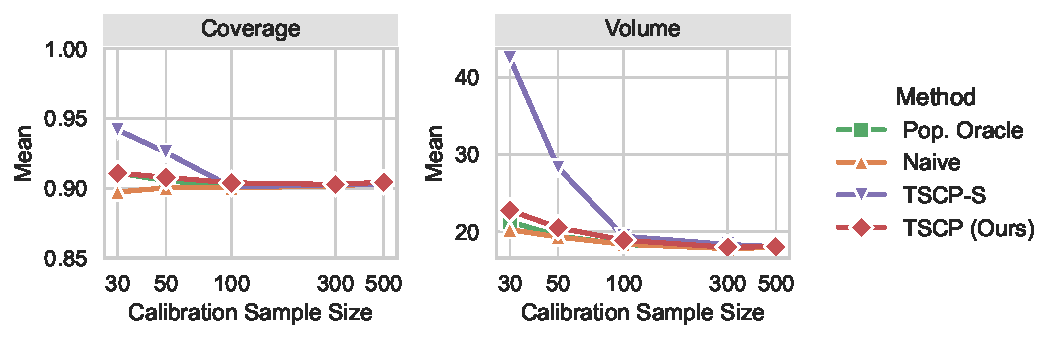
\includegraphics[width=0.9\textwidth]{figures/ours/ours_approximation_2d.pdf}
    \end{subfigure}
    \begin{subfigure}[b]{\textwidth}
        \centering
        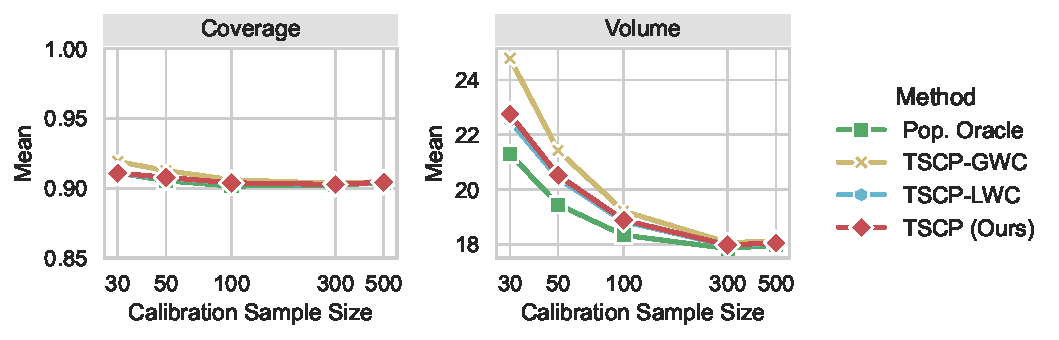
\includegraphics[width=0.9\textwidth]{figures/ours/ours_containment_2d.pdf}
    \end{subfigure}
    \caption{Performance of TSCP and alternative approaches on simulated data with $d=2$ targets and heterogeneous Laplace noise. The target coverage level is $90\%$. Results are averaged over $200$ trials. All methods achieve near-nominal coverage and approximate \emph{Pop.~Oracle} as the calibration sample size increases. TSCP tracks TSCP-LWC closely, with an almost indistinguishable average volume, highlighting the tightness of its rectangular enclosure.}
    \label{fig:approximation1}
\end{figure}

All methods compared in Figure~\ref{fig:approximation1} tend to approximate \emph{Pop.~Oracle} well as $n$ increases, with TSCP and TSCP-LWC being the two most stable and fastest approximations among all methods with theoretical coverage. These results also show that TSCP encloses the aggregated union TSCP-LWC very tightly, and that TSCP-GWC is conservative, though it still performs better than the data-splitting variant TSCP-S. Despite lacking a finite-sample coverage guarantee, the \emph{Naive} approach performs well, as also shown in Figure~\ref{fig:approximation2}.

\begin{figure}[!htbp]
    \centering
    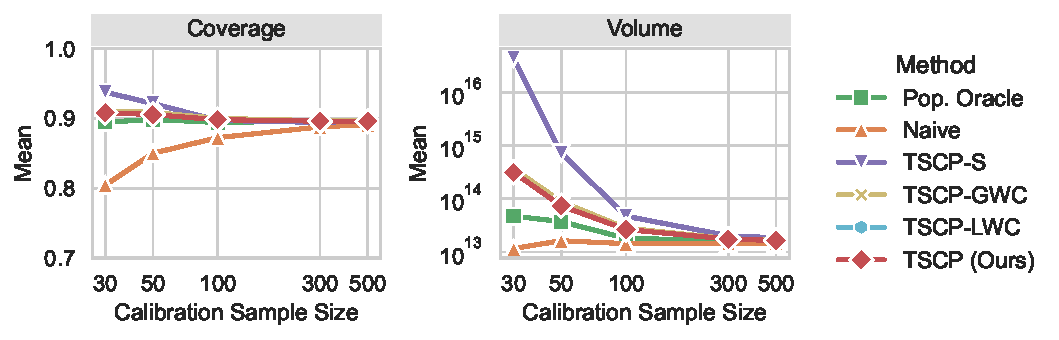
\includegraphics[width=0.9\textwidth]{figures/ours/ours_containment_10d.pdf}
    \caption{Performance of TSCP and alternative approaches on simulated data with $d=10$ targets. Other details are as in Figure~\ref{fig:approximation1}. TSCP-LWC is omitted from this figure due to its prohibitive cost with even moderately high-dimensional outcomes.}
    \label{fig:approximation2}
\end{figure}

Figure~\ref{fig:runtime} better highlights the prohibitive computational cost of TSCP-LWC, by reporting on the results of similar experiments where a small sample size is fixed, $|\mathcal{D}_{\mathrm{cal}}|=30$, while the outcome dimensions are gradually increased: $d \in \{2, 3, 4, 5, 10, 20, 30\}$.

\begin{figure}[!htbp]
    \centering
    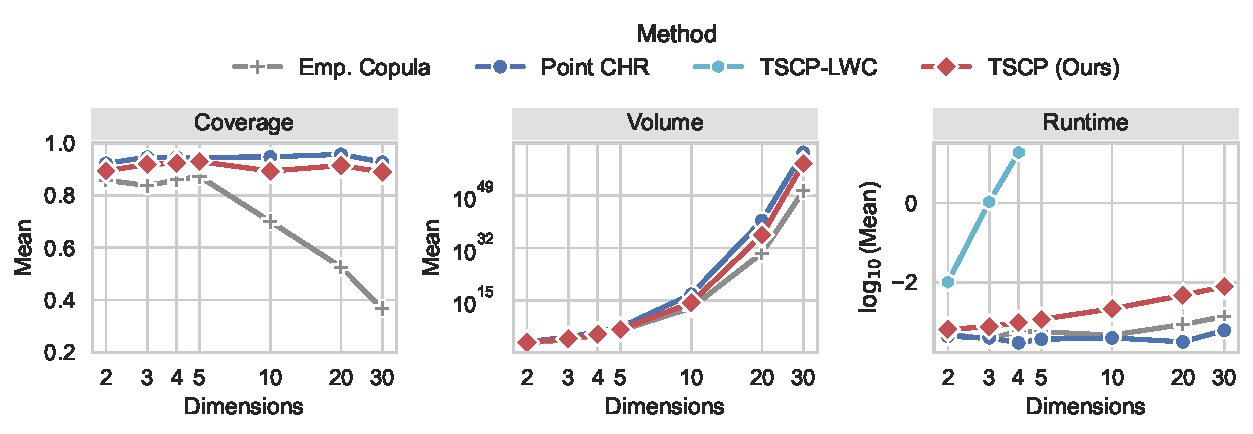
\includegraphics[width=\textwidth]{figures/ours/ours_runtime.pdf}
    \caption{Performance of TSCP and alternative approaches on simulated data with fixed sample size $|\mathcal{D}_{\mathrm{cal}}|=30$, as a function of the number of output dimensions $d$. Other details are as in Figure~\ref{fig:approximation1}. These results are averaged over $30$ independent repetitions. The runtime results are presented in seconds on a $\log_{10}$ scale. 
    The runtime of all methods except TSCP-LWC scales well with number of dimensions. TSCP-LWC is only applied when $d \in \{2,3,4\}$ due to the exponential growth of its runtime. }
    \label{fig:runtime}
\end{figure}

\clearpage
\subsection{Robustness to Heavy-Tailed Data} \label{app:hevy_tailed_simulation}


We test the performance of TSCP on simulated heavy-tailed data with $d=10$ outcomes and noise following a Student's-$t$ distribution; i.e., $Y_j \mid \mathbf X \sim f_j(\mathbf X) + \epsilon_j$ with $\epsilon_j \sim t_{\mathrm{DF}}$ and $\mathrm{DF} \in \{1.5,2,3\}$ degrees of freedom. 
For $1 < \mathrm{DF} \leq 2$, the Student's-$t$ distribution leads to residuals with infinite population variance, violating Assumption~\ref{eq:assumption-scores}. Nonetheless, TSCP continues to achieve the desired coverage level even in this extreme setting, although with some loss of informativeness.


\begin{figure}[!htbp]
     \centering
     \begin{subfigure}[b]{\textwidth}
         \centering
         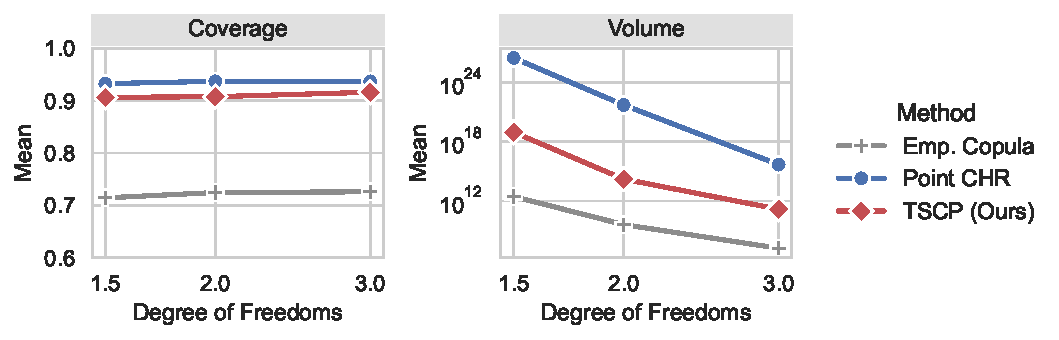
\includegraphics[width=0.9\textwidth]{figures/t/t_n30_10d.pdf}
         \caption{Small sample, $|\mathcal{D}_{\mathrm{cal}}|=30$. Output dimensions $d=10$.}
         \label{fig:t-n30-10d}
     \end{subfigure}
     \vfill
     \begin{subfigure}[b]{\textwidth}
         \centering
         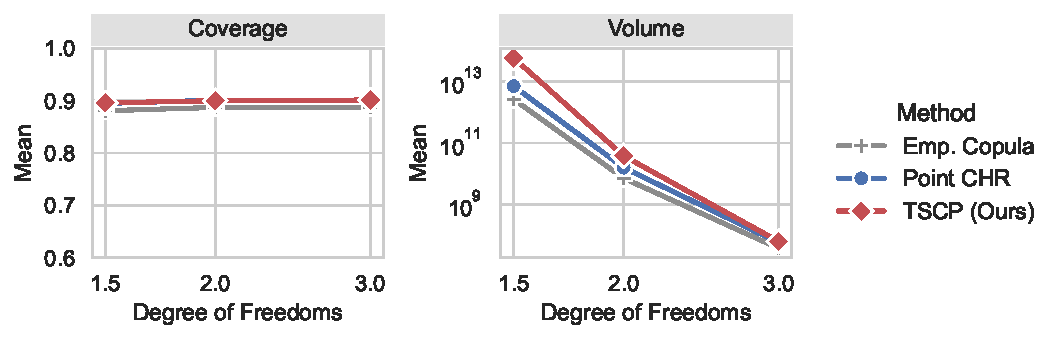
\includegraphics[width=0.9\textwidth]{figures/t/t_n500_10d.pdf}
         \caption{Large sample, $|\mathcal{D}_{\mathrm{cal}}|=500$. Output dimensions $d=10$.}
         \label{fig:t-n500-10d}
     \end{subfigure}
        \caption{Performance of the proposed TSCP method and other approaches on simulated data with noise following a Student's-$t$ distribution with varying degrees of freedom, using small (a) and large (b) sample sizes. The target coverage level is 0.9. All methods except \emph{Emp.~Copula} have near-nominal coverage in all settings. TSCP maintains valid marginal coverage even on very heavy-tailed data. In the small sample setting, Point CHR suffers more in terms of prediction set size due to its inefficient use of calibration data, although it can outperform TSCP in large samples.}
        \label{fig:t}
\end{figure}
 
% \begin{table}
%     \centering
%     \input{figures/t/t_n30_10d}
%     \caption{Performance on Student's-$t$ distribution with varying degree of freedoms on small sample size $|\mathcal{D}_{\mathrm{cal}}|=30$. This table contains all data used to generate Figure~\ref{fig:t-n30-10d} along with one standard deviation of the test coverage and volume over $200$ trials. Target coverage is $0.9$. Coverage below this target is highlighted in \textcolor{red}{red}. For volume, lower is better. Smallest volume size (among those with valid coverage) is highlighted in \textcolor{red}{red}. }
%     \label{tab:t-n30-10d}
% \end{table}

% \begin{table}
%     \centering
%     \input{figures/t/t_n500_10d}
%     \caption{Performance on Student's-$t$ distribution with varying degree of freedoms on large sample size $|\dataset_{\mathrm{cal}}|=500$. This table contains all data used to generate Figure~\ref{fig:t-n500-10d} along with one standard deviation of the test coverage and volume over $200$ trials. Target coverage is $0.9$. Coverage below this target is highlighted in \textcolor{red}{red}. For volume, lower is better. Smallest volume size (among those with valid coverage) is highlighted in \textcolor{red}{red}. Point CHR has the smallest volume while maintaing valid coverage when the degree of freedom is less than $3$, but when systematic outliers getting removed as the degree of freedom increases, our TSCP becomes the one with the smallest volume while maintaining valid coverage. }
%     \label{tab:t-n500-10d}
% \end{table}



%%% Local Variables:
%%% mode: latex
%%% TeX-master: "main"
%%% End:
